\documentclass{article}


\usepackage{arxiv}

\usepackage[utf8]{inputenc} % allow utf-8 input
\usepackage[T1]{fontenc}    % use 8-bit T1 fonts
\usepackage{hyperref}       % hyperlinks
\usepackage{url}            % simple URL typesetting
\usepackage{booktabs}       % professional-quality tables
\usepackage{amsfonts}       % blackboard math symbols
\usepackage{nicefrac}       % compact symbols for 1/2, etc.
\usepackage{microtype}      % microtypography
\usepackage{lipsum}
\usepackage{siunitx}
\usepackage[linesnumbered,ruled,vlined]{algorithm2e}
\usepackage{float}
\usepackage{amsmath}
\usepackage{enumerate}
\usepackage{cite}
\usepackage{xcolor}
\usepackage{graphicx}
\graphicspath{ {./images/} }

\newcommand{\note}[1]{\textbf{#1}}

\title{Your EA Report Title}


\author{
 Student Name 1\\
  Student number 1\\
  \texttt{1234@umail.leidenuniv.nl}\\
  %% examples of more authors
   \And
 Student Name 2\\
  Student number 2\\
  \texttt{2345@umail.leidenuniv.nl} \\
  %% \And
 %% Name \\
  %% Student number\\
  %% \texttt{email address} \\
  %% \AND
  %% Coauthor \\
  %% Affiliation \\
  %% Address \\
  %% \texttt{email} \\
  %% \And
  %% Coauthor \\
  %% Affiliation \\
  %% Address \\
  %% \texttt{email} \\
  %% \And
  %% Coauthor \\
  %% Affiliation \\
  %% Address \\
  %% \texttt{email} \\
}

\begin{document}
\maketitle
%% \begin{abstract}
%% Abstract of your report here.
%% \end{abstract}


% keywords can be removed
%\keywords{First keyword \and Second keyword \and More}


\section{Introduction}\label{sec:intro}
Consider the following items: 
\begin{itemize}
    \item Which version of GA did you choose to implement?
    \item Explain briefly how you performed hyperparameter tuning.
    \item Was the tuning effective, based on what you see from the tuning results?
    \item Anything else you would do in the assignment?
\end{itemize}

\section{Algorithms}
\label{sec:imple}

Outline your algorithms, algorithm parameters, and settings used for those parameters. 

\begin{algorithm}[!ht]
\SetAlgoLined
\SetKwInOut{Input}{Input}\SetKwInOut{Termination}{Termination}

\Input{Population size $\mu$\\Crossover probability $p_c$ \\etc.}
\Termination{The algorithm terminates when..}
\BlankLine

Initialization\;

\For{$i=1$ \KwTo $B$}{
Selection\;
Crossover\;
Mutation\;
}
\caption{Genetic Algorithm}\label{al:GA}
\end{algorithm}
 
You can explain the implementation in various ways, as long as you make them clear and understandable. If you prefer to explain your algorithm in pseudo-code, you could find an example (Algorithm \ref{al:GA}). Please ensure the algorithm and the results are reproducible from your description. \note{Note that if we cannot get the same results using the codes you submit, the PA grade is 0.} You can fix the random seed during your experiment and provide it to us so that we can avoid the different results caused by randomization. 

\section{Hyper-parameter tuning}
Describe the method and setting for the hyper-parameter tuning process.

\begin{algorithm}[!ht]
\SetAlgoLined
\SetKwInOut{Input}{Input}\SetKwInOut{Termination}{Termination}

\Input{Alg.~\ref{al:GA}, a tuning budget $B$, and objective functions }
\Termination{The algorithm terminates when..}
\BlankLine

\caption{Tuning procedure}\label{al:tuning}
\end{algorithm}

\section{Experimental Results}\label{sec:experi}

Description of the experiments and the results. Use the tables and figures generated from the IOHanalyzer. Make sure to present your results in a way that is convenient to the reader. \textbf{do not blindly include plots of all your experiments; try to combine information in figures and tables!} 

Figure \ref{fig:example} and \ref{fig:test} show examples of how to insert your figure in the report. Please also see the captions. Make sure you explain your figures properly in the captions.

\begin{figure}[!ht]
 \begin{center}    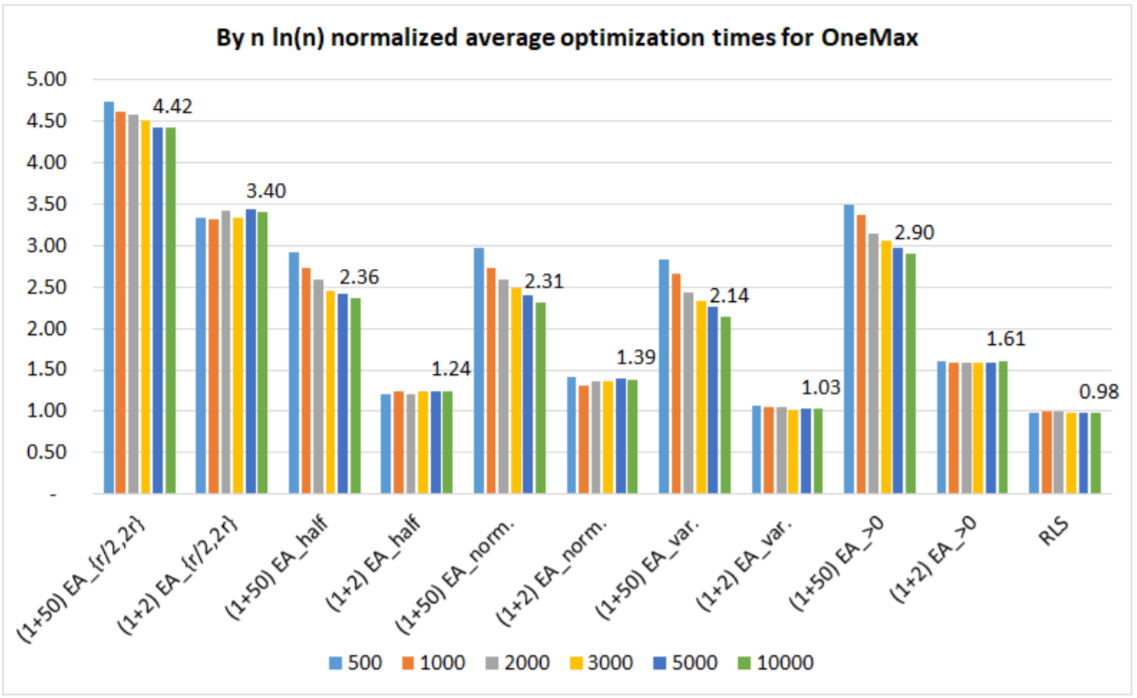
\includegraphics[width=0.95\textwidth]{example.png}
 \end{center}
 \caption{By $n\ln(n)$ normalized average optimization times for OneMax, for $n$ between 500 and 10 000. Displayed numbers are for $n = 10 000$ \cite{ye2019interpolating}.}
 \label{fig:example}
\end{figure}


\begin{figure}[!ht]
 \begin{center}    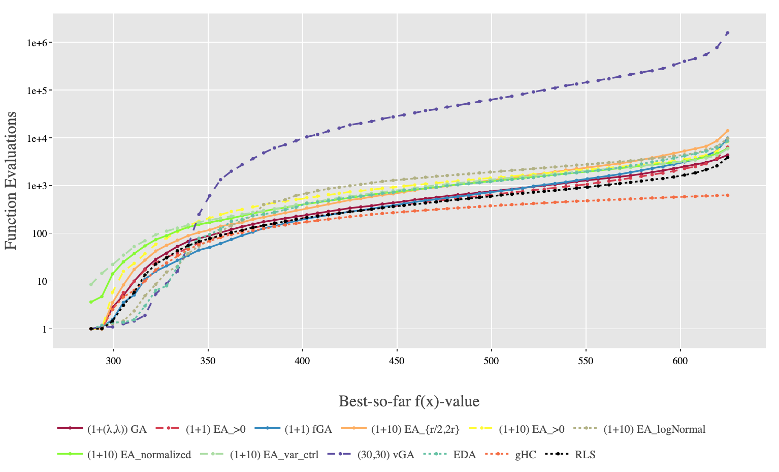
\includegraphics[width=0.95\textwidth]{best-so-far.png}
 \end{center}
 \caption{The fixed-target results of 11 algorithms. The figure is downloaded from IOHanalyzer.}
 \label{fig:test}
\end{figure}

\section{Discussion and Conclusion}\label{sec:dis&res}

Summarize the results and conclude your report. If you would like to put the main conclusions discussions as lists in this part, you can see an example below.

\begin{enumerate}[1)]
    \item We suggest using population size $\mu=x$ for the genetic algorithm to solve the problem.
    
    \item The genetic algorithm benefits from small mutation rates in solving the \textsc{NAS} problem. (Just an example, this may not be the truth.)
    
    \item We observe that the evolution strategy benefits from comma selection for solving the \textsc{NAS} problem. (Again, just an example).
\end{enumerate}
 
 \textbf{Tips:} Please put the references in the file \emph{references.bib} and cite them in the right line, like this \cite{hadash2018estimate}.

\bibliographystyle{unsrt}  
\bibliography{references}  


\end{document}
